\documentclass[11pt,a4paper]{article}
\usepackage[margin=1in]{geometry}
\usepackage[T1]{fontenc}
\usepackage{lmodern}
\usepackage{hyperref}
\usepackage{enumitem}
\usepackage{longtable}
\usepackage{array}
\usepackage{titlesec}
\usepackage{setspace}
\usepackage{xcolor}
\usepackage{fancyhdr}
\usepackage{amsmath}
\usepackage{graphicx}
\usepackage{float}
\usepackage{placeins}

\hypersetup{
  colorlinks=true,
  linkcolor=blue,
  urlcolor=blue
}

\setlength{\parskip}{0.20em}
\setlength{\parindent}{0pt}
\setstretch{1.12}
\pagestyle{fancy}
\fancyhf{}
\rhead{COMP4321 Final Project Report}
\lhead{Search Engine}
\cfoot{\thepage}
\setlength{\headheight}{14pt}

\titleformat{\section}{\large\bfseries}{\thesection}{0.6em}{}
\titleformat{\subsection}{\normalsize\bfseries}{\thesubsection}{0.6em}{}

\begin{document}

\begin{titlepage}
  \centering
  {\Large The Hong Kong University of Science and Technology\par}
  \vspace{1.2cm}
  {\LARGE \textbf{COMP4321 Web Search Engines}\par}
  \vspace{0.5cm}
  {\Large Final Project Report\par}
  \vspace{1.5cm}

  {\large Project Title: \textbf{Web-based Search Engine with Spider, Indexer, and Retrieval}\par}
  \vspace{1.0cm}

  \begin{tabular}{>{\raggedright\arraybackslash}p{0.32\linewidth}p{0.62\linewidth}}
    Course & COMP4321 Web Search Engines \\
    Semester & 2026 Spring \\
    Seed URL & \url{https://hitcslj.github.io/TestPages/testpage.htm} \\
    Indexed Pages & 300 \\
    Group No. & 25 \\
  \end{tabular}

  \vfill

  \begin{tabular}{>{\raggedright\arraybackslash}p{0.32\linewidth}p{0.62\linewidth}}
    Member 1 & SHAHEER, Muhammad (21026904) \\
    Member 2 & SAMI, Sufyan (20901389) \\
    Member 3 & PERYSHKO, Mira Eleanora (21333577) \\
  \end{tabular}

  \vfill
  {\large Submission Date: May 7, 2026\par}
\end{titlepage}

\section{Overall Design of the System}

\subsection{System Overview}
Our system contains four core modules:
\begin{enumerate}[leftmargin=1.5em]
  \item \textbf{Spider/Crawler}: Crawls pages using BFS from a seed URL and extracts links.
  \item \textbf{Indexer}: Performs stop-word removal, stemming, positional indexing, and metadata extraction.
  \item \textbf{Retrieval Engine}: Executes vector-space ranking with cosine similarity and phrase matching.
  \item \textbf{Web Interface (JSP)}: Accepts queries and renders ranked results in required format.
\end{enumerate}

\subsection{Data Flow}
\begin{enumerate}[leftmargin=1.5em]
  \item Spider fetches page and extracts title/body/links.
  \item Indexer transforms tokens (normalize $\rightarrow$ stop-word filter $\rightarrow$ stem).
  \item Indexed data is persisted to JDBM structures.
  \item Search engine reads indexes, computes scores, and returns top results.
  \item JSP pages present results with score, metadata, keywords, and parent/child links.
\end{enumerate}
This staged pipeline lets us validate each module independently during debugging and demo.
For example, crawl correctness is observed through \texttt{spider\_result.txt}, index
correctness through DB inspection, and ranking correctness through query outputs.

\section{File Structures Used in the Index Database}

All persistent data is stored in one JDBM RecordManager (\texttt{searchengine}) using multiple named HTrees.

\subsection{Core Mappings}
\begin{itemize}[leftmargin=1.5em]
  \item \texttt{url\_to\_pageID}: URL $\rightarrow$ pageID
  \item \texttt{pageID\_to\_url}: pageID $\rightarrow$ URL
  \item \texttt{word\_to\_wordID}: stem $\rightarrow$ wordID
  \item \texttt{wordID\_to\_word}: wordID $\rightarrow$ stem
\end{itemize}

\subsection{Indexes and Metadata}
\begin{itemize}[leftmargin=1.5em]
  \item \texttt{bodyIndex}: wordID $\rightarrow$ postings (pageID, tf, positions)
  \item \texttt{titleIndex}: wordID $\rightarrow$ postings (pageID, tf, positions)
  \item \texttt{forwardIndex}: pageID $\rightarrow$ (wordID $\rightarrow$ tf)
  \item \texttt{pageMetadata}: pageID $\rightarrow$ title, URL, last-modified, size, maxTF
\end{itemize}

\subsection{Link Graph and Counters}
\begin{itemize}[leftmargin=1.5em]
  \item \texttt{childLinks}: pageID $\rightarrow$ child pageIDs
  \item \texttt{parentLinks}: pageID $\rightarrow$ parent pageIDs
  \item \texttt{counters}: \texttt{pageCounter}, \texttt{wordCounter}
\end{itemize}
The schema combines both inverted and forward indexes. Inverted indexes are efficient for
retrieval and ranking, while the forward index supports fast top-keyword extraction for result
presentation. This dual design reduces query-time overhead and keeps UI rendering responsive.

\section{Algorithms Used}

\subsection{Breadth-First Crawling}
The crawler uses a queue-based BFS strategy and a visited set to avoid loops. URLs are mapped to IDs and link relations are stored bidirectionally (parent/child). Re-crawl skip logic is based on last-modified comparison.
BFS was chosen for predictable traversal from the seed and stable behavior under crawl limits
such as N=30 in hidden tests and N=300 for final indexing.

\subsection{Token Processing}
\begin{enumerate}[leftmargin=1.5em]
  \item Lowercase and remove non-alphabetic characters.
  \item Remove stop words from \texttt{stopwords.txt}.
  \item Apply Porter stemming.
  \item Store positions for phrase queries.
\end{enumerate}
The same normalization and stemming are applied on query-side input, ensuring retrieval parity
between indexed terms and query terms.

\subsection{Ranking Model}
For each term:
\[
  w_{d,t} = \frac{tf_{d,t}}{\max tf_d} \cdot idf_t,
  \quad
  idf_t = \log\left(\frac{N}{df_t}\right)
\]
Query and document vectors are compared with cosine similarity:
\[
  \text{score}(d,q)=\frac{\sum_t w_{d,t}w_{q,t}}
  {\|d\|\|q\|}
\]
In implementation, the query vector is built using the same idf values, and candidate
documents are produced from posting lists of query terms/phrases. The final list is sorted
in descending score order and truncated to top 50 as required by the specification.

\subsection{Title Boosting}
We add a bonus for title matches (term and phrase). This increases rank for pages where
query intent appears in title text. The title boost can be toggled at runtime for demo:
\texttt{SearchMain --no-title-boost ...} (CLI) and a checkbox in JSP UI. This allows direct
before/after comparison using the same query.
This design is easy to explain in demonstration: base relevance is first computed from body
content, then title evidence is added to prioritize pages whose titles directly match user intent.

\subsection{Phrase Search}
Phrase matching is implemented by checking adjacency in positional postings for both title
and body indexes. For a phrase of length $k$, if term 1 appears at position $p$, then term 2
must appear at $p+1$, ..., term $k$ at $p+k-1$ in the same document field. This supports
exact phrase lookup in both body and title.
In practice, this removes false positives from non-adjacent token matches and improves precision
for quoted queries.

\subsection{Bonus Feature Implemented}
\textbf{Excluded terms/phrases}:
\begin{itemize}[leftmargin=1.5em]
  \item \texttt{-term}
  \item \texttt{-"exact phrase"}
\end{itemize}
Documents containing excluded conditions are filtered out before ranking output. This is
integrated into query parsing and candidate filtering, so users can refine results without
changing the base ranking model. Example: \texttt{university -science} removes pages that
match \texttt{science}; \texttt{"hong kong" -"science park"} removes pages matching the
excluded phrase while preserving other phrase matches.
This bonus has low implementation risk but high demo value because users can immediately see
result set changes with and without exclusion constraints.

\section{Installation Procedure}

\subsection{Compile}
\begin{verbatim}
javac -cp .:htmlparser.jar:lib/jdbm-1.0.jar \
  IRUtilities/Porter.java StopStem.java Posting.java PageMetadata.java \
  DBManager.java Crawler.java Spider.java QueryParser.java \
  SearchEngine.java SearchMain.java TestProgram.java
\end{verbatim}

\subsection{Build 300-page DB}
\begin{verbatim}
rm -f searchengine.db searchengine.lg
java -cp .:htmlparser.jar:lib/jdbm-1.0.jar Spider \
  "https://hitcslj.github.io/TestPages/testpage.htm" 300
\end{verbatim}

\subsection{Run CLI Retrieval}
\begin{verbatim}
java -cp .:htmlparser.jar:lib/jdbm-1.0.jar SearchMain "computer science"
\end{verbatim}

\subsection{Run JSP UI on Tomcat}
Deploy \texttt{web/search.jsp}, \texttt{web/results.jsp}, \texttt{web/WEB-INF/web.xml}, class files, and required jars to Tomcat webapp directory. Then open:
\begin{verbatim}
http://localhost:8080/comp4321search/search.jsp
\end{verbatim}

\section{Testing and Results}

\subsection{Functional Tests}
\begin{itemize}[leftmargin=1.5em]
  \item 300-page indexing from required seed URL.
  \item Hidden-seed simulation with N=30 from empty DB.
  \item Re-run skip behavior validation.
  \item Query tests: single term, multi-term, phrase, zero-result, stop-word-only.
  \item Stemming parity: \texttt{run} vs \texttt{running}, \texttt{book} vs \texttt{books}.
  \item Bonus tests for excluded terms and phrases.
\end{itemize}
Observed behavior during test runs confirms that hidden-seed N=30 crawling completes in
demo-friendly time and immediate reruns index 0 additional pages when content is unchanged.

\begin{figure}[H]
  \centering
  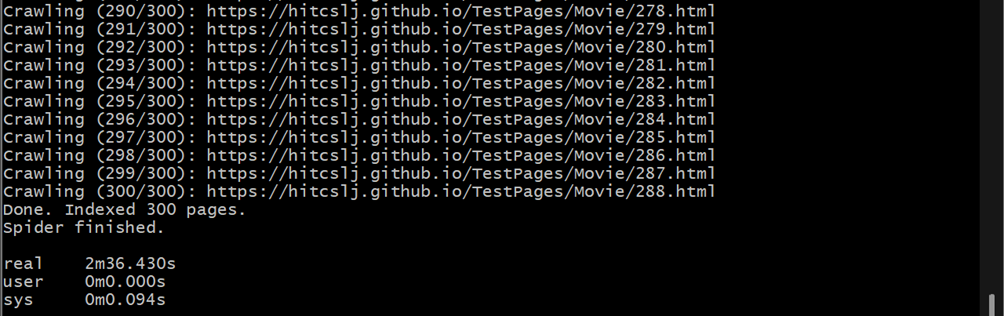
\includegraphics[width=0.96\linewidth]{screenshots/crawleroutput.png}
  \caption{Crawler output screenshot (N=300 indexing completion and runtime).}
\end{figure}

\begin{figure}[H]
  \centering
  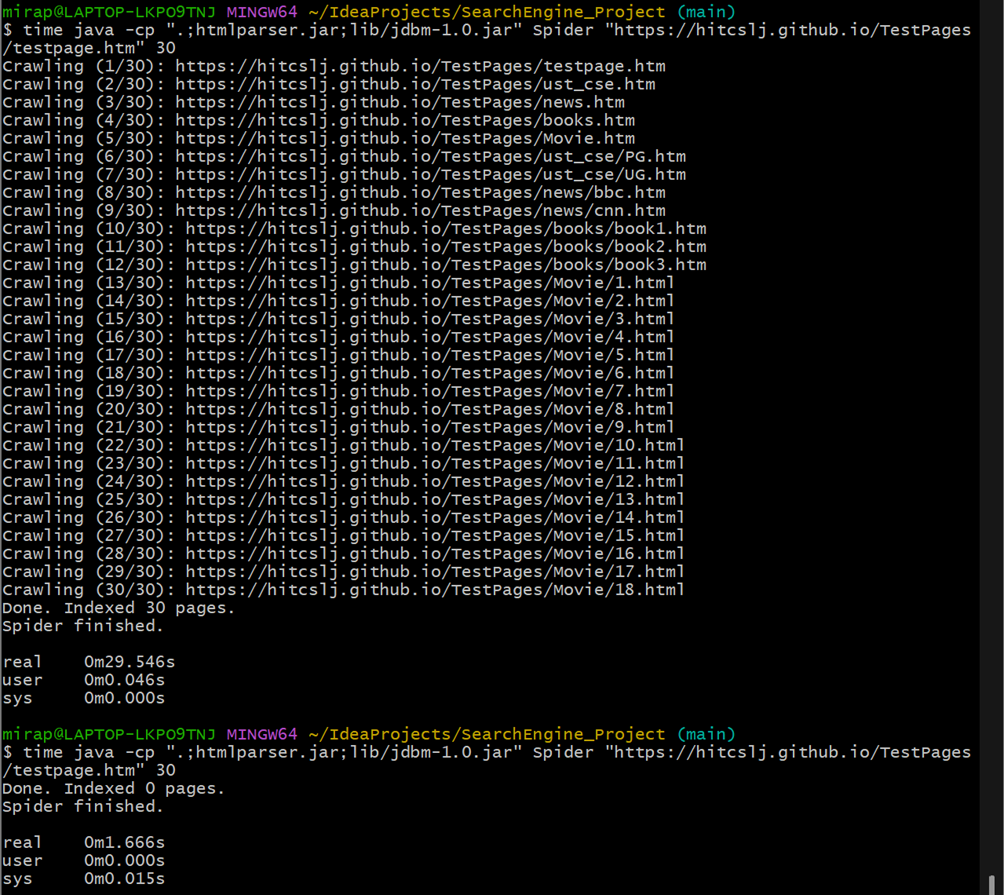
\includegraphics[width=0.96\linewidth]{screenshots/hiddenseedtest.png}
  \caption{Hidden-seed test screenshot (N=30 and rerun skip behavior).}
\end{figure}

\begin{figure}[H]
  \centering
  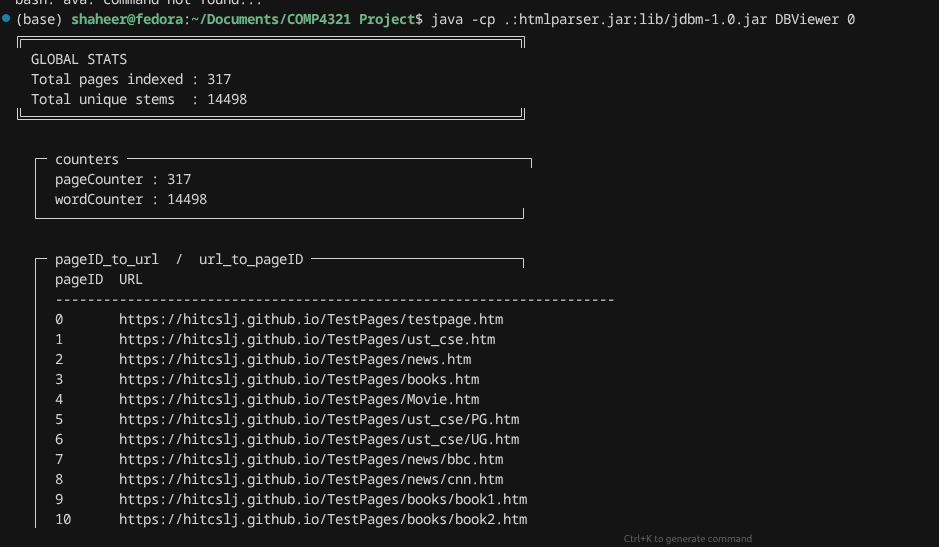
\includegraphics[width=0.94\linewidth]{screenshots/dbviewer.png}
  \caption{DB inspector output showing postings, term frequency, and positional data.}
\end{figure}

\begin{figure}[H]
  \centering
  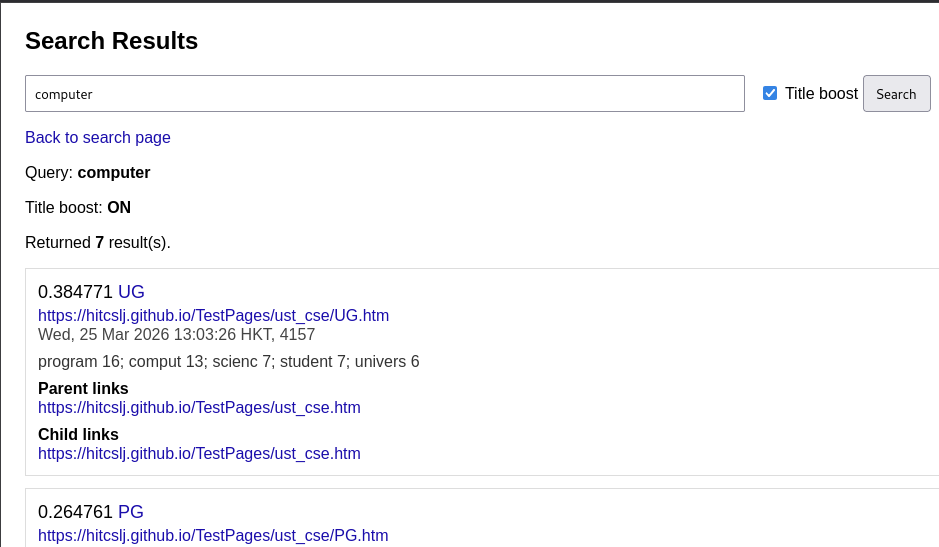
\includegraphics[width=0.96\linewidth]{screenshots/webUIoutput.png}
  \caption{Web UI result page showing score, title/URL hyperlinks, metadata, keywords, and parent/child links.}
\end{figure}

\begin{figure}[H]
  \centering
  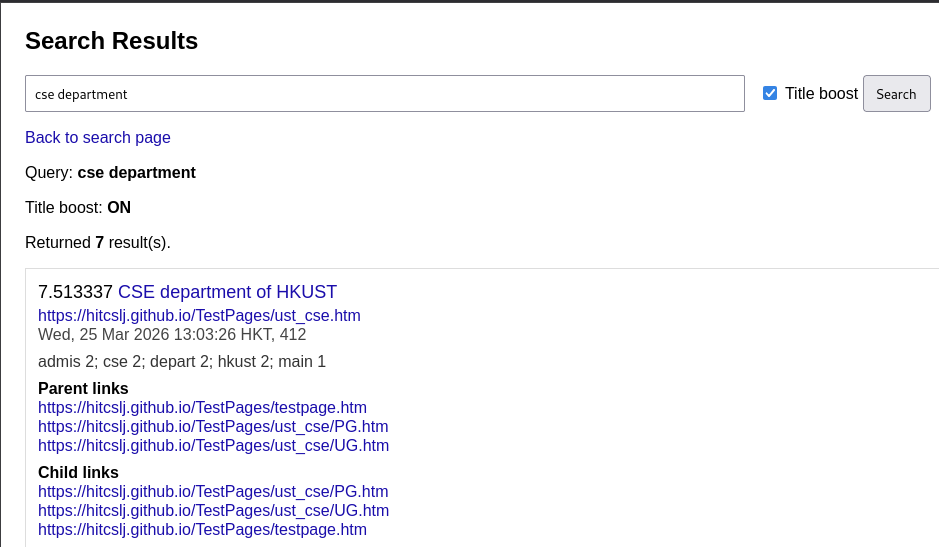
\includegraphics[width=0.92\linewidth]{screenshots/titlebooston.png}
  \caption{Title boost enabled.}
\end{figure}

\begin{figure}[H]
  \centering
  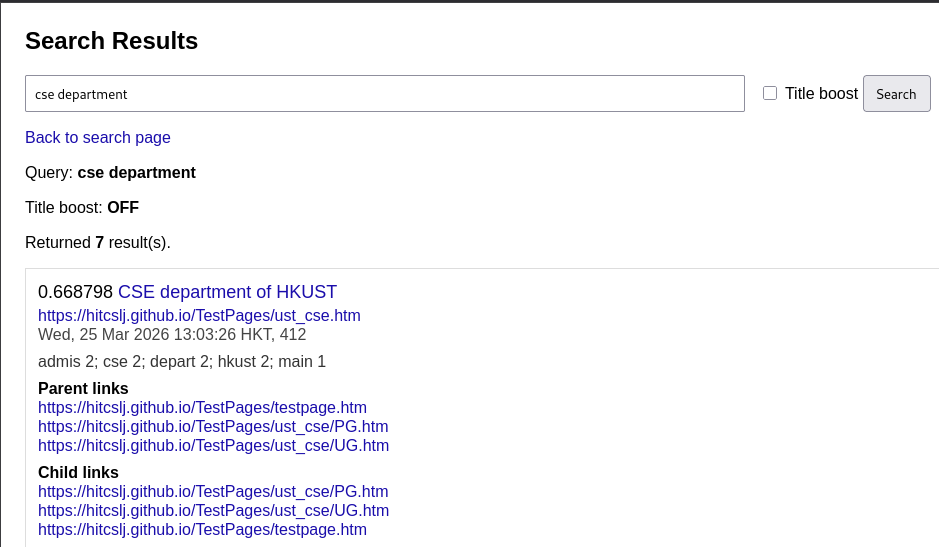
\includegraphics[width=0.92\linewidth]{screenshots/titleboostoff.png}
  \caption{Title boost disabled for the same query; score gap changes.}
\end{figure}

\begin{figure}[H]
  \centering
  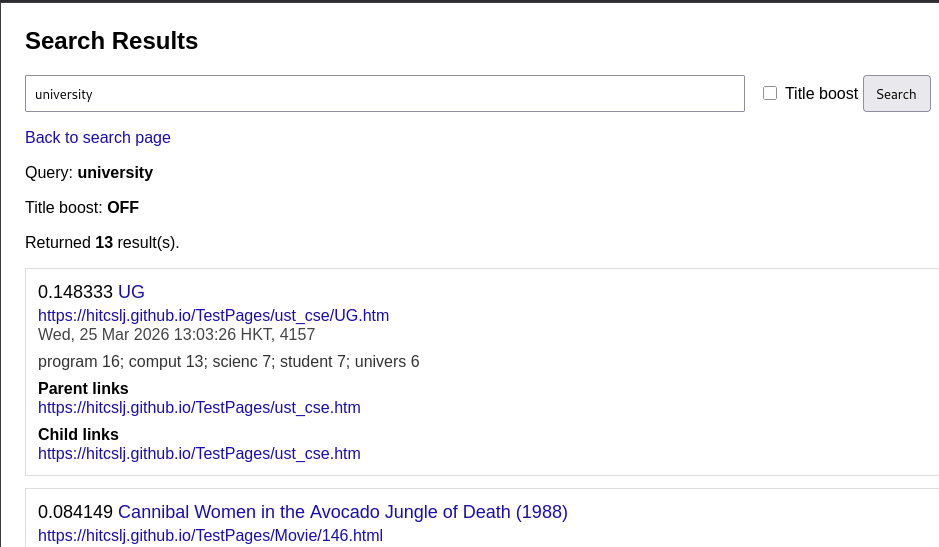
\includegraphics[width=0.92\linewidth]{screenshots/bonusfeature1.png}
  \caption{Bonus query example 1: excluded term filtering.}
\end{figure}

\begin{figure}[H]
  \centering
  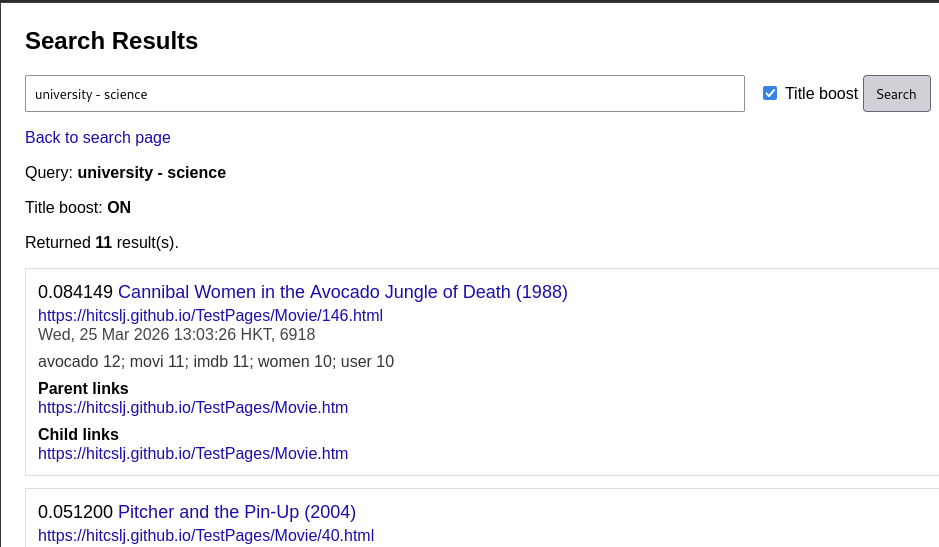
\includegraphics[width=0.92\linewidth]{screenshots/bonusfeature2.png}
  \caption{Bonus query example 2: excluded phrase filtering.}
\end{figure}
\FloatBarrier

\section{Conclusion}
\subsection{Strengths}
\begin{itemize}[leftmargin=1.5em]
  \item Complete end-to-end system from crawling to web retrieval.
  \item Proper phrase support through positional indexing.
  \item Clean separation of body/title indexes to support title emphasis.
  \item Practical bonus feature with clear demo value.
\end{itemize}

\subsection{Weaknesses}
\begin{itemize}[leftmargin=1.5em]
  \item Single-threaded crawler can be improved for throughput.
  \item Limited query language compared with production search engines.
  \item Basic UI focused on correctness over visual polish.
\end{itemize}

\subsection{Future Improvements}
\begin{itemize}[leftmargin=1.5em]
  \item Multi-threaded crawling with polite throttling.
  \item Better URL canonicalization and duplicate-content handling.
  \item Link-based ranking extension (e.g., PageRank).
  \item Enhanced UI interactions and result filtering controls.
\end{itemize}
Another practical enhancement is configurable DB path binding so CLI and servlet environments
can share the same index location without manual file copying.

\section{Contribution}
\begin{longtable}{|>{\raggedright\arraybackslash}p{0.28\linewidth}|>{\raggedright\arraybackslash}p{0.18\linewidth}|>{\raggedright\arraybackslash}p{0.46\linewidth}|}
\hline
\textbf{Member} & \textbf{Contribution} & \textbf{Main Responsibilities} \\
\hline
[SHAHEER, Muhammad (21026904)] & 33.3\% & Spider/crawling and link graph logic \\
\hline
[SAMI, Sufyan (20901389)] & 33.3\% & Indexing/database schema and retrieval implementation \\
\hline
[PERYSHKO, Mira Eleanora (21333577)] & 33.3\% & Web interface, testing, documentation, and demo prep \\
\hline
\end{longtable}

\vspace{0.5cm}
\textbf{Note:} Ensure total contribution percentages sum to 100\%.

\end{document}
